%%%%%%%%%%%%%%
% BASIC FORMATTING %
%%%%%%%%%%%%%%

\documentclass[11 pt]{article}
%\documentclass[10 pt]{amsart}

%LOAD VARIOUS PACKAGES
\usepackage{amsmath,amssymb,amsthm,amsfonts,graphicx,url,colordvi}
\usepackage{graphics,graphics,latexsym,multicol}
\usepackage{enumerate}

%SET MARGINS
\usepackage[margin = 1 in]{geometry} 
%\usepackage[left=1.5in,top=1.5in,right=1.5in,nohead,bottom=1.5in]{geometry}

%SET SPACING
\renewcommand{\baselinestretch}{1}


%%%%%%%%%%%%%%%%%%%%
% BUILD YOUR OWN SHORTCUTS %
%%%%%%%%%%%%%%%%%%%%


%MATH CHARACTER COMMANDS
\newcommand{\R}{\mathbb R} %REALS
\newcommand{\C}{\mathbb C} %COMPLEX
\newcommand{\N}{\mathbb N} %NATURAL NUMBERS
\newcommand{\Q}{\mathbb Q} %RATIONALS
\newcommand{\Z}{\mathbb Z} %INTEGERS

%LOWER CASE VECTORS v, x, AND b IN BOLDFACE
\newcommand{\vecv}{\mathbf v} 
\newcommand{\vecx}{\mathbf x}
\newcommand{\vecb}{\mathbf b}

%SYMBOL TAU IN BOLD
\newcommand{\tor}{\boldsymbol{\tau}}

%FORMAT THEOREMS
\newtheorem{theorem}{Theorem}[section]
\newtheorem{lemma}[theorem]{Lemma}
\newtheorem{conjecture}[theorem]{Conjecture}
\newtheorem{problemma}[theorem]{Problemma}
\newtheorem{proposition}[theorem]{Proposition}
\newtheorem{definition}[theorem]{Definition}
\newtheorem{corollary}[theorem]{Corollary}
\newtheorem{remark}[theorem]{Remark}
\newtheorem{example}[theorem]{Example}
\newtheorem{claim}{Claim}


%DEFINE NEW NAMED FUNCTIONS
\DeclareMathOperator{\rank}{rank}
\DeclareMathOperator{\Hom}{Hom}
\DeclareMathOperator{\conv}{conv}




%%%%%%%%%%%%%%%%
% MATH  ENVIRONMENTS %
%%%%%%%%%%%%%%%%


%INLINE EQUATION
% $f(x) = x^2$
% $\displaystyle f(x)=x^2$

%CENTERED EQUATION
% $$ f(x)=x^2 $$

%LABELED EQUATION. 
%(TO REFER TO THE EQUATION LATER IN TEXT TYPE "(\ref{quadratic})".)
%begin{equation}\label{quadratic}
% f(x)=x^2
%\end{equation}

%ALIGNED FORMULA WITHOUT LABELLING
%\begin{align*}
%f(x)&=x^2-2x+1 \\
%   &=(x-1)^2 \\
% 	&< 5.
%\end{align*}


%%%%%%%%%
% EXAMPLES %
%%%%%%%%%
 

%1. FRACTIONS AND RADICALS

% $\frac{x-1}{x+1}$
% $\sqrt[n]{x^2+1}$ 

%2. MATRIX COMMANDS

% $\begin{matrix}a & b \\ c & d \end{matrix}$
% $\begin{bmatrix}a & b \\ c & d \end{bmatrix}$
% $\begin{pmatrix}a & b \\ c & d \end{pmatrix}$

%3. INTEGRAL

% $\int_{x=0}{x=1}x^2 \ dx$

%4. PIECEWISE DEFINED FUNCTION

% $p(t)=\begin{cases} \frac{1}{2}, &\text{if $t \in [-1,1]$}; \\ 0, &\text{otherwise,} \end{cases}$


%%%%%%%%%%%%%%%
% FIGURES AND TABLES %
%%%%%%%%%%%%%%%


%FIGURES

%\begin{figure}[h]
%\hfil \scalebox{.5}{ \rotatebox{0}{ \includegraphics{c:/images/sampleimage.eps} }}  \hfil 
%\caption{ Sample figure }
%\end{figure}

%TABLE COMMANDS 

%\begin{tabular}{c|c} $x$ & $y$ \\ \hline a & b \\ c & d \\ e & f \ \end{tabular}

%MULTICOLUMN TABLE

%\begin{table}[h]
%\begin{center}
%\begin{tabular}{|c|c|c|c|c|c|c|} 
%\hline
%& \multicolumn{6}{c|}{Genotype of Parents}\\ \hline
%Genotype of Offspring & AA-AA & AA-Aa & AA-aa & Aa-Aa & Aa-aa & aa-aa \\ \hline 
%AA &  &  &  & &  &    \\ \hline
%Aa &  &  &  & &  &    \\ \hline
%aa &  &  &  & &  &    \\ \hline
%\end{tabular}
%\end{center}
%\end{table}


%%%%%%%%%%%%%
%  MISCELLANEOUS  %
%%%%%%%%%%%%%

  
%WEB URL
%\texttt{http://www.phy.syr.edu/courses/java-suite/crosspro.html} 

%TWO ALIGNED FORMULA COLUMNS
%\begin{alignat}{2}
%P_0(x)&=1, & \qquad P_1(x)&=x \notag \\
%P_2(x)&=\frac{1}{2}(3x^2-1), & \qquad P_3(x)&=\frac{1}{2}(5x^3-3x) \notag 
 % \end{alignat} 

%VARIABLE SPACED COLUMNS IN A TABLE
%\begin{tabular}{p{2.5in} p{2.5in}}
%	$\det(BA)$ &   $\det(A^{-1})$ \vspace{2in} \\
%	$\det(3B)$ &   $\displaystyle \det \left( \begin{bmatrix} 1 & 2 & 4 \\ 2 & 0 & -2 \\ 1 & 2 & 2 \end{bmatrix} \right)$ 
%	\end{tabular}



%%%%%%%%%%%%%%%
% START OF DOCUMENT %
%%%%%%%%%%%%%%%


\title{A Wavelet Based Search Engine}
\author{Samuel Tay}
\date{05/06/2011}


\begin{document}


\maketitle

\section{Introduction}

\indent\indent The purpose of this project is to use wavelets to design a search engine for images. The details of the project are outlined by Aboufadel and Schlicker [1]. Given an image, we define a \emph{feature vector}, which contains much of the information from the image, but will be much smaller than the matrix representation of the image. Then we define a distance between these vectors, which ultimately will be how we determine if images are similar to each other. We will use the Haar wavelets to construct the feature vectors, and although the project outlined in [1]  is for 16-by-16 pixel images, this project uses 256-by-256 pixel images.
%Does it really convert into matrix representation? Wording?
\section{Image Boxes}

\indent\indent The first step in creating a feature vector is to construct an image box. As stated above, the images we are using are 256-by-256 pixels, or equivalently $2^8$-by-$2^8$. We first import four images into Matlab, converting them into their matrix representations, converting their entries to double format, and converting the images to grayscale. The four images are shown below.

\begin{center}
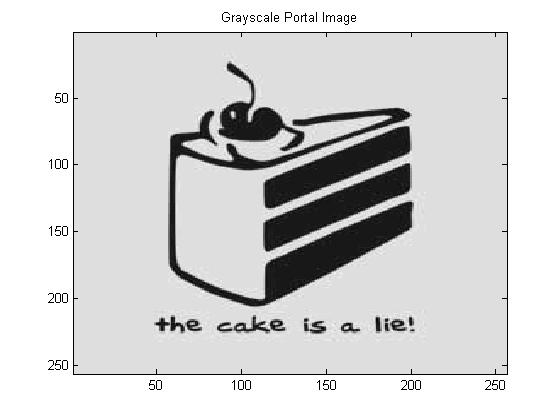
\includegraphics[width=3.2in]{Figure_1.jpg} 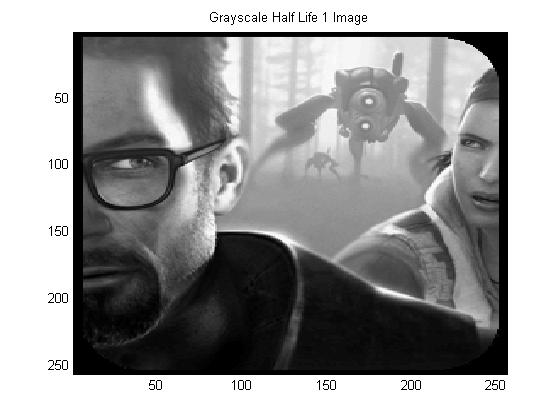
\includegraphics[width=3.2in]{Figure_2.jpg}\\
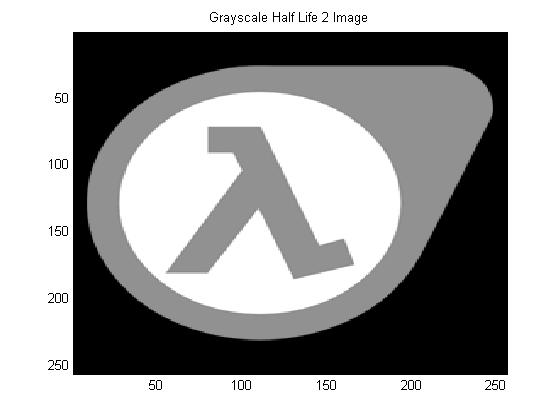
\includegraphics[width=3.2in]{Figure_3.jpg} 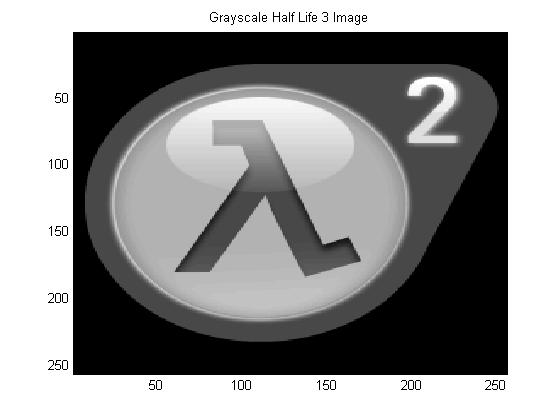
\includegraphics[width=3.2in]{Figure_4.jpg}
\end{center}

\indent To construct the image boxes, we will be processing each image using the Haar wavelets. Since the matrix representation $J$ of each image is $2^8\times 2^8$, we can consider each column of the matrix as a signal in $V_8$. Processing a signal in $V_n$ with the Haar wavelets is projecting the signal onto $V_{n-1}$ and $V_{n-1}^\perp$, and as a consequence of the Orthogonal Decomposition Theorem, this is ultimately just going to change the basis with which we describe the signal [1,2]. This change of basis can be achieved by a simple averaging and differencing matrix [2], which we'll call $P$.

%DO I NEED TO SAY MORE ABOUT P?
Since we are considering each column of the image matrix $J$ as a signal in $V_8$, we can multiply $PJ$ to simultaneously process all of the columns of $J$. Let $J_1$ be the resulting matrix, which consists of two new $2^7\times 2^8$ matrices $J_h$ and $J_g$ such that $$J_1=PJ=\begin{bmatrix}J_h\\J_g\end{bmatrix}_{2^8 \times 2^8}.$$ Now the columns of $J_h$ are average approximations of the columns of $J$ in $V_7$, and the columns of $J_g$ are the residuals of these approximations in $V_7^\perp$. Applying this procedure in Matlab to our original images yield the processed images below.

\begin{center}
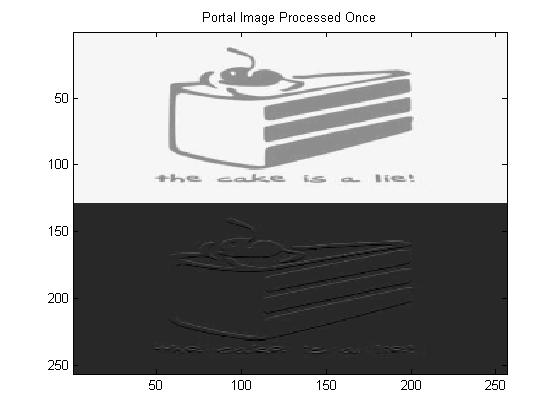
\includegraphics[width=3.2in]{Figure_5.jpg} 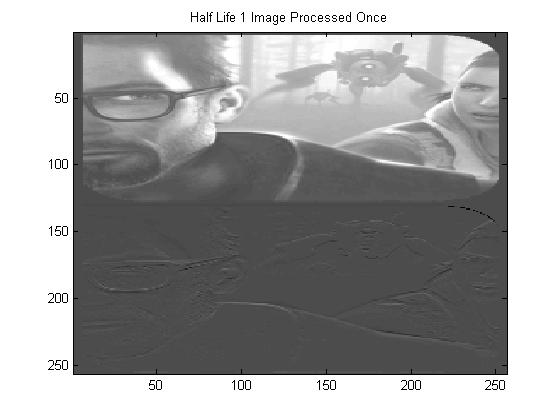
\includegraphics[width=3.2in]{Figure_6.jpg}\\
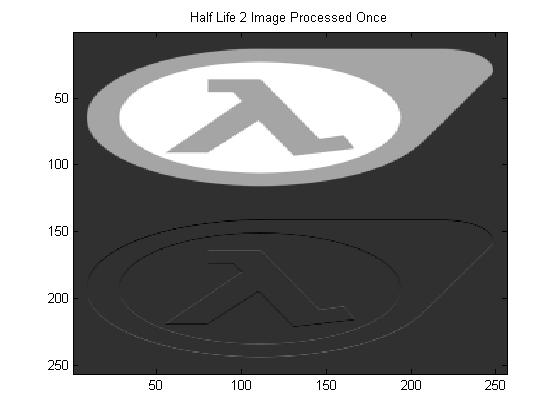
\includegraphics[width=3.2in]{Figure_7.jpg} 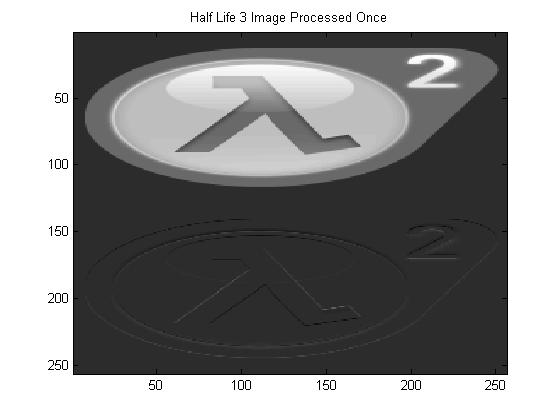
\includegraphics[width=3.2in]{Figure_8.jpg}
\end{center}

We can tell that these images fit with our abstract description: the top half is an average approximation, and the bottom half is the difference, or residual, between the original image and the approximation. We also see that since our original images were square, $J_h$ cannot be the average approximation of the entire original image, since $J_h$ is squished down. We still need to process across the rows of $J_h$ and $J_g$, which is why this process is often referred to as a \emph{two-dimensional wavelet transform} [1]. To process the rows, we can process the columns of $J_h^T$ and of $J_g^T$, which are in $V_8$. This might sound contradictory, but recall that we processed the \emph{columns} of $J$ into $V_7$ and $V_7^\perp$. While the rows of $J_h$ and $J_g$ are certainly not the original rows of $J$, they are still separate signals from the columns of $J_h$ and $J_g$, and thus can be independently thought of as signals in $V_8$.

Again, we simultaneously process the columns of $J_h^T$ and $J_g^T$ by multiplying these matrices by the same change of basis matrix $P$. Then $$PJ_h^T=\begin{bmatrix}J_{hh}^T\\J_{hg}^T\end{bmatrix}\implies (PJ_h^T)^T=\begin{bmatrix}J_{hh}^T\\J_{hg}^T\end{bmatrix}^T=\begin{bmatrix}J_{hh} & J_{hg}\end{bmatrix}\text{, and}$$ $$PJ_g^T=\begin{bmatrix}J_{gh}^T\\J_{gg}^T\end{bmatrix}\implies (PJ_g^T)^T=\begin{bmatrix}J_{gh}^T\\J_{gg}^T\end{bmatrix}^T=\begin{bmatrix}J_{gh} & J_{gg}\end{bmatrix}.$$

We processed the transpose of the rows of $J_h$ and $J_g$, so we need to take the transpose of these processed signals when substituting them back into $J_1$ for $J_h$ and $J_g$. However, now that we have processed twice, we'll call this matrix $J_2$, such that $$J_2=\begin{bmatrix}J_{hh} & J_{hg}\\J_{gh} & J_{gg}\end{bmatrix}.$$ The rows of $J_h$ and $J_g$, each signals in $V_8$, have undergone the same process as the columns of $J$, such that the rows of $J_{hh}$ and $J_{gh}$ are the average approximations in $V_7$ of the rows of $J_h$ and $J_g$ respectively. Similar to before, the rows of $J_{hg}$ and $J_{gg}$ are the residuals of the respective approximations in $V_7^\perp$. The twice processed images are shown below.

\begin{center}
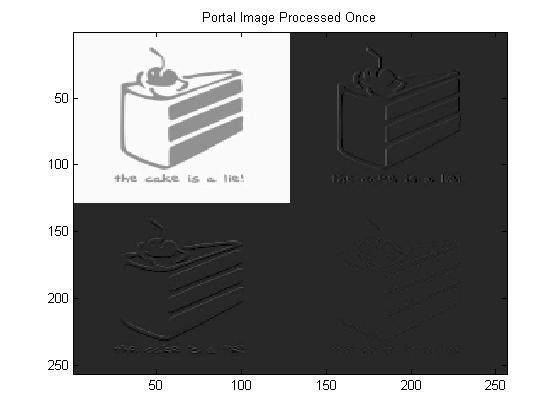
\includegraphics[width=3.2in]{Figure_9.jpg} 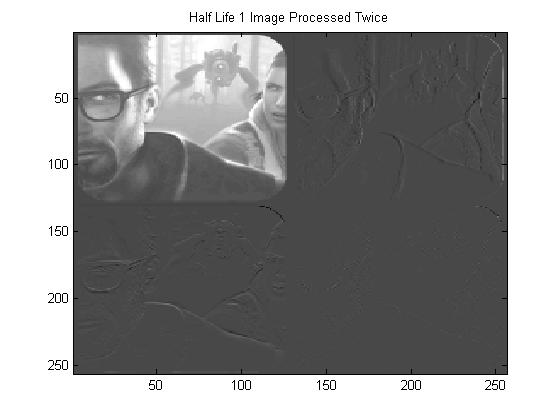
\includegraphics[width=3.2in]{Figure_10.jpg}\\
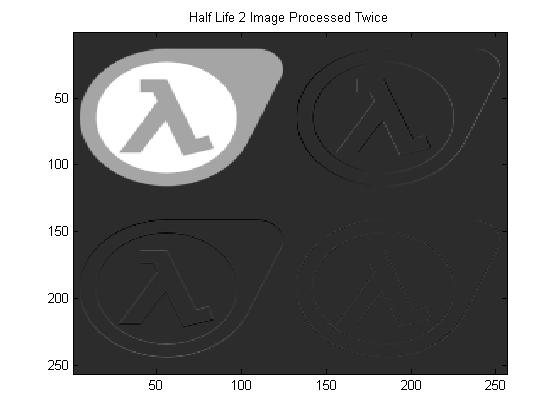
\includegraphics[width=3.2in]{Figure_11.jpg} 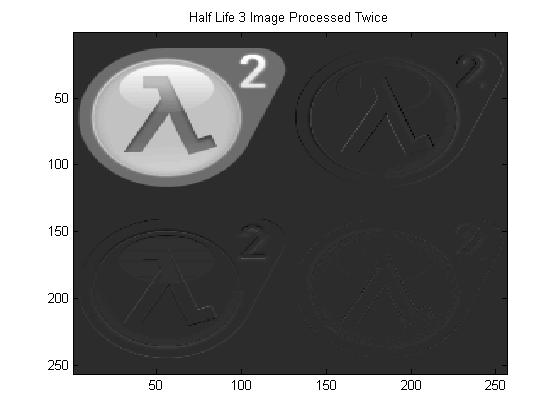
\includegraphics[width=3.2in]{Figure_12.jpg}
\end{center}

These image boxes fit with our description of their construction; notice that the top left image, corresponding to $J_{hh}$, is just a smaller approximation to the original image. This is because $J_{hh}$ is the average approximation of $J_h$, which was the average approximation of $J$, but it is now squished in the other direction to be square again. Thus the entries of $J_{hh}$ come directly from averaging. Also notice that the bottom right image is the faintest; this is because it corresponds to $J_{gg}$, which is the residual left over after approximating the first residual, which we'd expect to be very faint in comparison to the other parts of the image box. The two-dimensional wavelet transform usually continues with applying this same procedure to $J_{hh}$, but this image box is sufficient for creating the feature vector.

\section{The Feature Vector}

\indent\indent We are almost in the position to create the feature vector. However, first we must apply quantile thresholding to $J_{hh}$. To do this, we use Matlab to string out the entries of $J_{hh}$ into a vector $\mathbf{v}$. Since $J_{hh}$ is $128\times 128$, $\mathbf{v}$ will be in $\mathbb{R}^{16384}$. We then sort the vector and find the $16384\cdot \frac{1}{4} = 4096^{th}$ entry and set it equal to the threshold $\lambda$. Now 25\% of the entries of $J_{hh}$ are less than or equal to $\lambda$. Let $C$ be the matrix $J_{hh}$ after setting all entries less than or equal to $\lambda$ to zero.

Now we define the feature vector $\mathbf{f} \in\mathbb{R}^{16640}$. (Note that $16640=128^2+2\cdot 128$.) The first $128^2=16384$ entries are simply the entries of $C$, such that the first 128 entries of $\mathbf{f}$ are the entries of the first row, the next 128 entries of $\mathbf{f}$ are the entries of the second row, and so on up until the last entry: $$f_1=c_{1,1},f_2=c_{1,2},\cdots, f_{128}=c_{1,128},$$ $$f_{128+1}=c_{2,1}, f_{128+2}=c_{2,2},\cdots, f_{2\cdot128}=c_{2,128},$$ $$\vdots$$ $$f_{128\cdot127+1}= c_{128,1},f_{128\cdot 127+2}=c_{128,2},\cdots, f_{128^2}=c_{128,128}.$$ Then the next $2\cdot 128=256$ entries of $\mathbf{f}$ are the diagonals of $J_{hg}$ and $J_{gh}$, such that $$f_{128^2+1}=j_{{hg}_{1,1}}, f_{128^2+2}=j_{{hg}_{2,2}}, \cdots, f_{128^2+128}=j_{{hg}_{128,128}},$$ and $$f_{128^2+128+1}=j_{{gh}_{1,1}}, f_{128^2+128+2}=j_{{gh}_{2,2}}, \cdots, f_{128^2+2\cdot 128}=j_{{gh}_{128,128}}.$$
This takes care of all of the 16640 entries of $\mathbf{f}$, so we have successfully defined the feature vector. We compute the feature vectors of our images in Matlab, but since each is in $\mathbb{R}^{16640}$, we won't list them out here; instead, refer to the appendix containing Matlab code.

In building an image search engine, the first thing we need to do is determine how we are going to tell if an image is similar to another image. Consider the feature vector: it contains at least 75\% of the entries of the approximated image $J_{hh}$, and as seen in the image boxes above, this is a very good approximation to the original image. Most if not all of the distinct features of the original image are captured, while only tiny detail definitions are lost. So even with just these entries, $\mathbf{f}$ already has enough information to represent 75\% of almost all of the distinct features of the original image (in fact, since many of the entries of $J_{hh}$ might have already been zero, it can potentially represent much more than 75\% of $J_{hh}$). It also contains the diagonals of $J_{hg}$ and $J_{gh}$, which means it has some general information about the residuals; in particular it contains information about what happens when we process the image, which is unique to the image itself, and thus is useful information for describing the image. With all of this in mind, it makes sense that if images have similar feature vectors, the images will be similar.

To compare feature vectors, we can define a weighted distance between them:
$$d(\mathbf{u},\mathbf{v})=\sum_{i=1}^{16384} w_1|u_i-v_i| + \sum_{i=16385}^{16640}w_2 |u_i-v_i|$$ where $w_1$ and $w_2$ are weights that can be chosen arbitrarily. However, since the most important information describing the original image is in the first 16384 entries that come from $C$ (recall 75\% of which are from $J_{hh}$), it makes sense to have $w_1$ larger than $w_2$. We will experiment with a few different choices of these weights in the next section. Given that we have chosen them well, we can sketch out how a search engine would work based on these feature vectors.

\section{Results}
\indent\indent We compute the distances between each of the feature vectors of our four images, first using the weights $w_1=1$ and $w_2=\frac{1}{4}$. We expect that the distance between feature vectors of the Half Life 2 and Half Life 3 images will be small relative to the rest of the distances, since these images are very similar. (If you're curious, one is the logo for the first Half-Life videogame, and the other is for the sequel - hence the exponent two.) Let $\mathbf{f}_i$ denote the feature vector of the $i^{th}$ image, ordered as they are listed in the paper. The results are listed below.

$$d(\mathbf{f}_1,\mathbf{f}_2) = 1.6062\cdot 10^6$$
$$d(\mathbf{f}_1,\mathbf{f}_3) = 1.7715\cdot 10^6$$
$$d(\mathbf{f}_1,\mathbf{f}_4) = 1.2447\cdot 10^6$$
$$d(\mathbf{f}_2,\mathbf{f}_3) = 1.3353\cdot 10^6$$
$$d(\mathbf{f}_2,\mathbf{f}_4) = 1.1256\cdot 10^6$$
$$d(\mathbf{f}_3,\mathbf{f}_4) = 0.6292\cdot 10^6$$

Our expectations are met in the last value comparing the similarity between images Half Life 2 and Half Life 3. The distance between the two feature vectors is significantly less than any other distance computed; its about one half the value of the next smallest distance which is between the Half Life 1 and Half Life 3 images. Although, comparing the images by eye, I would have expected the difference between Half Life 2 and Half Life 3 to be even lower than this. The resulting distances when using $w_1=1$ and $w_2=\frac{1}{10}$ are shown below.

$$d(\mathbf{f}_1,\mathbf{f}_2) = 1.6032\cdot 10^6$$
$$d(\mathbf{f}_1,\mathbf{f}_3) = 1.7687\cdot 10^6$$
$$d(\mathbf{f}_1,\mathbf{f}_4) = 1.2416\cdot 10^6$$
$$d(\mathbf{f}_2,\mathbf{f}_3) = 1.3319\cdot 10^6$$
$$d(\mathbf{f}_2,\mathbf{f}_4) = 1.1223\cdot 10^6$$
$$d(\mathbf{f}_3,\mathbf{f}_4) = 0.6292\cdot 10^6$$

The results are pretty much the same, but considering that only $256/16640\approx 1.5\%$ of the terms in the sum are from the diagonals, this isn't too surprising. For the sake of curiosity, the distances resulting from $w_1=w_2=1$ are shown below.

$$d(\mathbf{f}_1,\mathbf{f}_2) = 1.6215\cdot 10^6$$
$$d(\mathbf{f}_1,\mathbf{f}_3) = 1.7855\cdot 10^6$$
$$d(\mathbf{f}_1,\mathbf{f}_4) = 1.2606\cdot 10^6$$
$$d(\mathbf{f}_2,\mathbf{f}_3) = 1.3527\cdot 10^6$$
$$d(\mathbf{f}_2,\mathbf{f}_4) = 1.1419\cdot 10^6$$
$$d(\mathbf{f}_3,\mathbf{f}_4) = 0.6292\cdot 10^6$$

This actually tells us something significant about the Half Life 2 and Half Life 3 images. Note that we have increased $w_2$ and held $w_1$ constant, so every distance computed with these values should be greater than the distances from the previous weights. This is true in all of the distances except between Half Life 2 and Half Life 3, for which the distance has remained constant while we've changed $w_2$ twice. This leads us to believe that the two have identical or at least nearly identical diagonals in $J_{hg}$ and $J_{gh}$. Also, since the distance between these two has remained constant while the others have risen, the relative size of this distance with respect to the other distances is less than the size we obtained with the previous weights, which is a good result, as these images are near identical. So, we could choose these as our weights for now, even though we did argue before that $w_2$ should be less than $w_1$. For a very informed choice on these two values, we would need to sample a much larger selection of images.

\section{Building an Image Search Engine}

\indent\indent Unfortunately, the search engine at this level of sophistication would be very limited for a number of reasons. The feature vectors that we have defined are dependent on the construction of an image box that, at this level, is only defined for square images that have sizes $2^n$-by-$2^n$ pixels. We are also working with grayscale images, but it wouldn't be so hard to extend our ideas to color images in an RGB format; we could bump up to three dimesions (i.e., feature vector would be the same length but have three columns), or we could compute a feature vector that simply has its length tripled, for the entries for R,G, and B.

Suppose however that we are in a situation where a search engine just needs to take input of a grayscale $2^n$-by-$2^n$ image and find another grayscale $2^n$-by-$2^n$ image similar to the input. The engine could compute the feature vector exactly as we did in Matlab, and then compute the feature vectors of the images of whatever database it has. After computing the distances between the input feature vector and the database feature vectors, the engine could sort the results in ascending order, and then output a list of the corresponding images from the database in the same order. Then, hopefully, the first image would be most similar to the input. If we are checking to see if the image is already within the database, we would use this search engine to save time and memory, as a computer would have a much easier time comparing the distance between two feature vectors than comparing two full images. For example, in our case, the distance between feature vectors is a sum of 16640 terms. If we were to define a distance comparing every entry of the image matrix, this would be a sum of $256^2=65536$ terms. So this primitive search engine can definitely be a useful tool in certain situations.

\section{Conclusion}
\indent\indent Although we have only tested our method of determining image similarity between four images, we can tell that the basic idea works from the comparison between Half Life 2 and Half Life 3. We do not know however how well this method works in comparing, say fifty very similar images. If we took a bunch of different Half Life Logo images, we'd hope that the Half Life logos from the first game would be more similar to each other than to Half Life 2 logos (the image with the exponent 2 on $\lambda$). If we wanted to expand on this search engine and refine it a bit, we could compare a large number of similar images by eye, and tweak the distance definition until it yields the results we need it to. If needed we can expand the feature vector by adding on more values from the other parts of the image boxes, or perhaps if it turns out to work equally as well, we can throw out more of the $J_{hh}$ values to save time and memory. We can make all of these improvements with relative ease, as the Matlab code is versatile and so well commented. So we conclude this project with the primitive search engine being sufficient in certain situations, knowing that if it needs to be improved, we can certainly expand the ideas to a more complex search engine.








\end{document}

%% modify matlab code for any vectors to v=zeros(1,n)

%as up above, ask if matrix representation conversion is correct

%ask if the paper is awkward having the search engine ideas before results

%% ask if there's too much information about image box construction
 %=====> ask if i need to say more about change of basis P
 %=====> ask if the whole transposed j-hh stuff is too much









